\documentclass[a4paper,12pt]{article}
\usepackage{blindtext}
\parskip=12pt 

\usepackage[T1]{fontenc}
\usepackage{lmodern}
\usepackage[utf8]{inputenc}
\usepackage{booktabs}

\usepackage{amsmath}
\usepackage{amsthm}
\usepackage{amssymb}

\usepackage{mathrsfs}
\usepackage{mathtools}

\usepackage{epsfig}
\usepackage{epstopdf}

\usepackage{bigints}
\usepackage{lastpage} 
\usepackage{comment} 
\usepackage{setspace}
\usepackage{enumerate}
\usepackage{parskip}

\usepackage{kbordermatrix}



\usepackage{float,lscape}
\usepackage{array}
\newcolumntype{L}[1]{>{\raggedright\let\newline\\\arraybackslash\hspace{0pt}}m{#1}}
\newcolumntype{C}[1]{>{\centering\let\newline\\\arraybackslash\hspace{0pt}}m{#1}}
\newcolumntype{R}[1]{>{\raggedleft\let\newline\\\arraybackslash\hspace{0pt}}m{#1}}
\usepackage{dcolumn}
\usepackage[top=1in, bottom=1in, left=1in, right=1in]{geometry}
%\renewcommand{\baselinestretch}{1.50}\normalsize
\usepackage{multirow}

\usepackage{verbatim} 
\usepackage{lipsum}
\usepackage{setspace}
\usepackage{nth}

\usepackage{framed}

\usepackage{bm}

\usepackage{relsize}


\usepackage{graphicx}
\usepackage{xcolor}

\usepackage{algorithmicx}
\usepackage{algorithm}
\usepackage{algpseudocode}

%\setcounter{tocdepth}{2}
\usepackage{abstract}
\usepackage[round]{natbib}
\usepackage{hyperref}

\usepackage{lscape}
\usepackage{pdflscape}

\newcommand{\E}{\mathop{\mbox{\sf E}}} 
\newcommand{\Var}{\mathop{\mbox{\sf Var}}}     % ISE
\newcommand{\Cov}{\mathop{\mbox{\sf Cov}}}     % ISE
\newcommand{\QQ}{\mathop{\mbox{\sf Q}}}     % ISE
\newcommand{\PP}{\mathop{\mbox{\sf P}}}     % ISE

\theoremstyle{plain}
\newtheorem{lem}{Lemma}[subsection]
\newtheorem{thm}{Theorem}[section]
\theoremstyle{definition}
\newtheorem{exmp}{Example}[subsection]
\newtheorem{defn}{Definition}[subsection]
\newtheorem{prop}{Proposition}[subsection]


\definecolor{darkgreen}{HTML}{007F00}
\definecolor{dblue}{HTML}{000099}

\newcolumntype{.}{D{.}{.}{-1}}

\usepackage{booktabs,mathptmx,siunitx}
\sisetup{input-symbols = {()},  % do not treat "(" and ")" in any special way
         group-digits  = false}
         
\usepackage{caption,fixltx2e}
\usepackage[flushleft]{threeparttable}

\begin{document}




\newpage

\section{Descriptive information about the data}

\subsection{Basic information}

In this section, we describe the 1st month of the OPRA data as well as some of their relevant characteristics.

In Table \ref{table_desc} some descriptive statistics are listed. The number of quotes and trades after applying the cleaning algorithm in Section 2 is provided. 

Some examples of the traded contracts are shown in Figures \ref{cntrt_pics_1} - \ref{cntrt_pics_4}. It can be seen that different contracts and underlyings vary significantly in terms of prevailing spreads, amount of transactions, dynamics of different exchanges and in time.

In the fourth panel of Table \ref{table_desc} it can be seen that the majority of traded contracts has maturity 1 week to 1 month in most of the cases, except for securities GOOG, XLE, K and BLK.

In the last panel of Table \ref{table_desc}, trades' directions are determined using an algorithm similar to that of \citet{lee_ready}. It can be described as follows.

For each trade price $P_t$ for a certain contract, do the following:

\begin{enumerate}
\item
determine the prevailing bid and ask quotes $Q_t^B$ and $Q_t^A$ (1st BBO quotes at or immediately preceding time $t$);
\item
compute the prevailing mid-quote $Q_t^M = (Q_t^B + Q_t^A)/2$;
\item
then decide:
	\begin{enumerate}
	\item
	if $P_t > Q_t^M$, then the trade at time $t$ is buyer-initiated (BI)
	\item
	if $P_t < Q_t^M$, then the trade at time $t$ is seller-initiated (SI)
	\item
	if $P_t = Q_t^M$, then decide based on the following:
		\begin{enumerate}
		\item
		if $P_t < P_{t-1}$, then the trade is SI
		\item
		if $P_t > P_{t-1}$, then the trade is BI
		\item
		if $P_t = P_{t-1}$, then one should sequentially check the differences between $P_t$ and $P_{t-2}, \ldots,  P_1$ until the first such difference is strictly smaller (SI) or larger (BI) than zero;
		\end{enumerate}
	\end{enumerate}
\item
if no condition from the above is satisfied, the the trade direction cannot be determined (UI).
\end{enumerate}

As follows from Table \ref{table_desc}, in most of the cases the number of buyer-initiated trades is larger than of those which are seller-initiated. 

It must be noted that we do not include contracts which are "trades-only" into the calculation as these would make impossible the use of the algorithm above.


\subsection{Liquidity measures}

We further calculate a number of liquidity measures for contracts on the given underlying securities, proposed, e.g., in \citet{huang_stoll}, \citet{hasbrouck}, \citet{goyenko_et_al}. The liquidity measures we consider are divided into 2 categories:

\begin{enumerate}
\item
spread measures: Effective Spread, Realized Spread;
\item
price impact measures: $\lambda$ Price Impact, 5-Minute Price Impact.
\end{enumerate}

The spread measures are intended to measure relationships either between trade prices and prevailing BBO mid-quotes at a given time or between trade prices at different time points. The price impact measures capture liquidity implications of transactions on the market.

The first measure, Effective Spread, is defined as follows:
\begin{equation}
ES_t \stackrel{\operatorname{def}}{=} 2 \cdot |\log(P_t) - \log(Q^M_t)|,
\end{equation} 
where $P_t$, $Q^M_t$ are as defined above.

The second measure, Realized Spread, is written in the following way:
\begin{equation}
RS_t \stackrel{\operatorname{def}}{=} \left\{ \begin{array}{ll}
              2 \cdot \left\{\log(P_t) - \log(P_{t+5})\right\}, & \mbox{if the $t$th trade is BI}\\
              2 \cdot \left\{\log(P_{t+5}) - \log(P_t)\right\}, & \mbox{if the $t$th trade is SI},\end{array} \right.
\end{equation}
where $P_{t+5}$ is the price of the trade 5 minutes after the $t$th trade.

The next measure, $\lambda$ Price Impact, is a a regression-based liquidity effect measure: it is defined as the slope coefficient of the following equation without a constant:
\begin{equation}
r_k = \lambda \cdot S_k + u_k,
\end{equation} 
where the log-return $r_k$ is computed for the $k$th 5-minute period, $u_k$ is the error term; $S_k$ is the signed square-root dollar volume:
\begin{equation}
S_k \stackrel{\operatorname{def}}{=} \sum_{t=1}^{T_k} Sign(V_t^k)\sqrt{V_t^k},
\end{equation} 
where $T_k$ is the number of trades in the $k$th 5-minute period, $V_t^k$ is the dollar volume of the $t$th trade in the $k$th interval, and
\begin{equation}
Sign(V_t^k) \stackrel{\operatorname{def}}{=} \left\{ \begin{array}{ll}
              1, & \mbox{if the $t$th trade in the $k$th interval is BI}, \\
              0,& \mbox{if the $t$th trade in the $k$th interval is UI},  \\
              -1, & \mbox{if the $t$th trade in the $k$th interval is SI}. \end{array} \right.
\end{equation}

The last price impact measure, 5-Minute Price Impact, is written as follows:
\begin{equation}
PI_t \stackrel{\operatorname{def}}{=} \left\{ \begin{array}{ll}
              2 \cdot \left\{\log(Q^M_{t+5}) - \log(Q^M_t)\right\}, & \mbox{if the $t$th trade is BI}\\
              2 \cdot \left\{ \log(Q^M_t) - \log(Q^M_{t+5})\right\}, & \mbox{if the $t$th trade is SI},\end{array} \right.
\end{equation}
where $Q^M_{t+5}$ is the midpoint of the BBO bid and ask quotes prevailing 5 minutes after the $t$th trade.

These liquidity measures are computed for each contract which has 2 or more trades in it. Contracts with trades only (without quotes) are also excluded due to the lack of quote entries. Descriptive statistics presented in Table \ref{table_liq}, are calculated over 20 days and all eligible contracts for each underlying security in the 1st month of data. Statistics on the eligible contracts are given in the bottom panel of Table \ref{table_liq}. 

From Table \ref{table_liq} follows an obvious result that options on more actively traded stocks such as SPY, AAPL, GOOG produce lower values of spread liquidity indicators with average Effective Spread being equal to 0.053, 0.047 and 0.058, respectively which is still much higher than monthly and annual averages obtained by \citet{goyenko_et_al} who used stock data in the NYSE TAQ database in the period from 1993 to 2005.

Interestingly enough, comparing a security with a relatively high amount of option trade and quote entries such as XLE, with a relatively illiquid one such as K, we find that their Effective and Realized spread measures are very close to each other. Also XLE has fewer trades than, e.g., XOM while having a higher amount of quote records.

Consistent with previous studies such as \citet{goyenko_et_al}, none of the spread or price impact indicators are of the same order of magnitude as the $\lambda$ price impact measure. In terms of interpretation, the $\lambda$ Price Impact for SPY at its median value 249 means that a \$10,000 buy order would move the log price by approximately $\sqrt{10,000} \times 249 \times 10^{-6} = 0.0249$, i.e., 2.5\%. Median values of $\lambda$ Price Impact obtained here are on average an order of magnitude larger than those presented in  \citet{goyenko_et_al} which is due to the fact that options normally have much smaller prices than the underlying stocks. 

As the next step in this descriptive study, one could perform analysis similar to that of  \citet{goyenko_et_al}, who tests the hypothesis that low-frequency liquidity measures can reliably estimate high-frequency benchmark indicators. 

\newpage

\vspace*{\fill}
\begin{figure}[H]
\begin{center}
 \minipage{0.45\textwidth}
 \includegraphics[width=\linewidth]{figures/contract_pics/SPY_top.png}
 \endminipage
 \hspace{3mm}
 \minipage{0.45\textwidth}
 \includegraphics[width=\linewidth]{figures/contract_pics/SPY_middle.png}
 \endminipage\\
 \vspace{5mm}
 \minipage{0.45\textwidth}
 \includegraphics[width=\linewidth]{figures/contract_pics/AAPL_top.png}
 \endminipage
 \hspace{3mm}
 \minipage{0.45\textwidth}
 \includegraphics[width=\linewidth]{figures/contract_pics/AAPL_middle.png}
 \endminipage\\
 \vspace{5mm}
 \minipage{0.45\textwidth}
 \includegraphics[width=\linewidth]{figures/contract_pics/GOOG_top.png}
 \endminipage
 \hspace{3mm}
 \minipage{0.45\textwidth}
 \includegraphics[width=\linewidth]{figures/contract_pics/GOOG_middle.png}
 \endminipage\\
 \vspace{5mm}
 \minipage{0.45\textwidth}
 \includegraphics[width=\linewidth]{figures/contract_pics/EA_top.png}
 \endminipage
 \hspace{3mm}
 \minipage{0.45\textwidth}
 \includegraphics[width=\linewidth]{figures/contract_pics/EA_middle.png}
 \endminipage
\end{center}
\vspace{-3mm}
\caption{\footnotesize Dynamics of selected contracts on various underlyings on 20150105: bid prices as solid, ask prices as dashed lines, trades as dots; colors denote different exchanges; dynamics of the underlyings in yellow} 
\label{cntrt_pics_1}
\end{figure}
\vspace*{\fill}

\newpage

\vspace*{\fill}
\begin{figure}[H]
\begin{center}
 \minipage{0.45\textwidth}
 \includegraphics[width=\linewidth]{figures/contract_pics/XLK_top.png}
 \endminipage
 \hspace{3mm}
 \minipage{0.45\textwidth}
 \includegraphics[width=\linewidth]{figures/contract_pics/XLK_middle.png}
 \endminipage\\
  \vspace{5mm}
 \minipage{0.45\textwidth}
 \includegraphics[width=\linewidth]{figures/contract_pics/XOM_top.png}
 \endminipage
 \hspace{3mm}
 \minipage{0.45\textwidth}
 \includegraphics[width=\linewidth]{figures/contract_pics/XOM_middle.png}
 \endminipage\\
  \vspace{5mm}
 \minipage{0.45\textwidth}
 \includegraphics[width=\linewidth]{figures/contract_pics/CVX_top.png}
 \endminipage
 \hspace{3mm}
 \minipage{0.45\textwidth}
 \includegraphics[width=\linewidth]{figures/contract_pics/CVX_middle.png}
 \endminipage\\
  \vspace{5mm}
 \minipage{0.45\textwidth}
 \includegraphics[width=\linewidth]{figures/contract_pics/MPC_top.png}
 \endminipage
 \hspace{3mm}
 \minipage{0.45\textwidth}
 \includegraphics[width=\linewidth]{figures/contract_pics/MPC_middle.png}
 \endminipage
\end{center}
\vspace{-3mm}
\caption{\footnotesize Dynamics of selected contracts on various underlyings on 20150105: bid prices as solid, ask prices as dashed lines, trades as dots; colors denote different exchanges; dynamics of the underlyings in yellow} 
\label{cntrt_pics_2}
\end{figure}
\vspace*{\fill}

\newpage

\vspace*{\fill}
\begin{figure}[H]
\begin{center}
 \minipage{0.45\textwidth}
 \includegraphics[width=\linewidth]{figures/contract_pics/XLE_top.png}
 \endminipage
 \hspace{3mm}
 \minipage{0.45\textwidth}
 \includegraphics[width=\linewidth]{figures/contract_pics/XLE_middle.png}
 \endminipage\\
  \vspace{5mm}
 \minipage{0.45\textwidth}
 \includegraphics[width=\linewidth]{figures/contract_pics/PG_top.png}
 \endminipage
 \hspace{3mm}
 \minipage{0.45\textwidth}
 \includegraphics[width=\linewidth]{figures/contract_pics/PG_middle.png}
 \endminipage\\
  \vspace{5mm}
 \minipage{0.45\textwidth}
 \includegraphics[width=\linewidth]{figures/contract_pics/WMT_top.png}
 \endminipage
 \hspace{3mm}
 \minipage{0.45\textwidth}
 \includegraphics[width=\linewidth]{figures/contract_pics/WMT_middle.png}
 \endminipage\\
  \vspace{5mm}
 \minipage{0.45\textwidth}
 \includegraphics[width=\linewidth]{figures/contract_pics/XLP_top.png}
 \endminipage
 \hspace{3mm}
 \minipage{0.45\textwidth}
 \includegraphics[width=\linewidth]{figures/contract_pics/XLP_middle.png}
 \endminipage
\end{center}
\vspace{-3mm}
\caption{\footnotesize Dynamics of selected contracts on various underlyings on 20150105: bid prices as solid, ask prices as dashed lines, trades as dots; colors denote different exchanges; dynamics of the underlyings in yellow} 
\label{cntrt_pics_3}
\end{figure}
\vspace*{\fill}

\newpage

\vspace*{\fill}
\begin{figure}[H]
\begin{center}
 \minipage{0.45\textwidth}
 \includegraphics[width=\linewidth]{figures/contract_pics/JPM_top.png}
 \endminipage
 \hspace{3mm}
 \minipage{0.45\textwidth}
 \includegraphics[width=\linewidth]{figures/contract_pics/JPM_middle.png}
 \endminipage\\
  \vspace{5mm}
 \minipage{0.45\textwidth}
 \includegraphics[width=\linewidth]{figures/contract_pics/BAC_top.png}
 \endminipage
 \hspace{3mm}
 \minipage{0.45\textwidth}
 \includegraphics[width=\linewidth]{figures/contract_pics/BAC_middle.png}
 \endminipage\\
  \vspace{5mm}
 \minipage{0.45\textwidth}
 \includegraphics[width=\linewidth]{figures/contract_pics/BLK_top.png}
 \endminipage
 \hspace{3mm}
 \minipage{0.45\textwidth}
 \includegraphics[width=\linewidth]{figures/contract_pics/BLK_middle.png}
 \endminipage\\
  \vspace{5mm}
 \minipage{0.45\textwidth}
 \includegraphics[width=\linewidth]{figures/contract_pics/XLF_top.png}
 \endminipage
 \hspace{3mm}
 \minipage{0.45\textwidth}
 \includegraphics[width=\linewidth]{figures/contract_pics/XLF_middle.png}
 \endminipage
\end{center}
\vspace{-3mm}
\caption{\footnotesize Dynamics of selected contracts on various underlyings on 20150105: bid prices as solid, ask prices as dashed lines, trades as dots; colors denote different exchanges; dynamics of the underlyings in yellow} 
\label{cntrt_pics_4}
\end{figure}
\vspace*{\fill}

\newpage

\begin{landscape}
\begin{table}[ht!]
  \centering
  \caption{Entries' statistics}
  \vspace{-0mm}
 \scalebox{0.55}{
 \bgroup
 \def\arraystretch{1.0}
    \begin{tabular}{@{}l C{2.3cm} C{2.3cm} C{2.3cm} C{2cm} C{2cm} C{2cm} C{2cm} C{2cm} C{2cm} C{2cm} C{2cm} C{1.5cm} C{2cm} C{2cm} C{2cm} C{2cm} C{2cm}@{}}
    \hline \hline
    \multicolumn{1}{c}{\multirow{2}{2cm}{\centering \textbf{  }}} & \multicolumn{17}{c}{\textbf{Underlying stocks}} \\
    \multicolumn{1}{c}{} & \multicolumn{1}{c}{\textbf{SPY}} & \multicolumn{1}{c}{ \textbf{AAPL} } & \multicolumn{1}{c}{ \textbf{GOOG} } & \multicolumn{1}{c}{ \textbf{EA} } &  \multicolumn{1}{c}{ \textbf{XLK} } &  \multicolumn{1}{c}{ \textbf{XOM} } &  \multicolumn{1}{c}{ \textbf{CVX} } & \multicolumn{1}{c}{ \textbf{MPC} } & \multicolumn{1}{c}{ \textbf{XLE} } & \multicolumn{1}{c}{ \textbf{PG} } & \multicolumn{1}{c}{ \textbf{WMT} } & \multicolumn{1}{c}{ \textbf{K} } & \multicolumn{1}{c}{ \textbf{XLP} } & \multicolumn{1}{c}{ \textbf{JPM} } & \multicolumn{1}{c}{ \textbf{BAC} } & \multicolumn{1}{c}{ \textbf{BLK} } & \multicolumn{1}{c}{ \textbf{XLF} } \\
\hline
& \multicolumn{17}{c}{\textbf{Number of records (before cleaning)}} \\
Avg       & 700,838,009 & 301,575,942 & 73,543,546  & 15,184,625 & 9,489,613  & 36,198,297 & 28,728,799 & 5,215,386 & 59,890,142 & 23,723,427 & 22,802,939 & 745,353 & 8,778,407  & 43,001,824 & 36,051,422 & 3,166,838 & 11,930,495 \\
Std Dev   & 139,414,541 & 78,014,816  & 17,064,430  & 4,269,292  & 2,406,511  & 7,548,864  & 5,085,071  & 1,290,710 & 11,537,807 & 8,134,120  & 6,288,729  & 120,562 & 2,341,311  & 8,747,138  & 6,725,070  & 724,910  & 2,642,094  \\
Median    & 694,355,725 & 310,310,810 & 71,363,687  & 14,629,507 & 8,729,688  & 34,021,556 & 27,206,324 & 5,066,729 & 58,010,337 & 24,989,843 & 23,184,688 & 718,706 & 8,477,310  & 41,790,218 & 34,030,353 & 3,139,884 & 11,100,126 \\
Min       & 409,607,244 & 159,094,428 & 45,479,752  & 9,744,870  & 5,399,868  & 24,735,171 & 21,143,683 & 3,245,001 & 45,196,390 & 9,543,493  & 12,224,635 & 574,871 & 4,851,901  & 25,718,345 & 23,281,419 & 1,968,863 & 6,549,215  \\
Max       & 984,010,543 & 417,942,352 & 113,190,636 & 23,388,291 & 13,105,051 & 49,712,308 & 38,714,736 & 8,314,240 & 84,261,758 & 38,230,503 & 33,970,789 & 981,853 & 13,133,224 & 59,398,468 & 49,911,031 & 5,340,371 & 17,999,368 \\
\hline
& \multicolumn{17}{c}{ \textbf{ Number of trades (after cleaning) } } \\
Avg       & 80,476     & 78,298     & 8,078      & 607      & 462      & 3,846     & 2,979     & 405     & 3,635     & 1,728     & 1,699     & 127    & 375      & 4,117     & 9,895     & 157     & 1,388     \\
Std Dev   & 15,585     & 27,043     & 3,932      & 643      & 125      & 1,028     & 1,084     & 261     & 1,223     & 742      & 623      & 59     & 179      & 1,941     & 3,724     & 79      & 449      \\
Median    & 80,004     & 72,670     & 6,637      & 424      & 456      & 3,820     & 2,828     & 301     & 3,277     & 1,513     & 1,515     & 122    & 337      & 3,443     & 8,869     & 115     & 1,321     \\
Min       & 44,787     & 45,928     & 4,947      & 185      & 224      & 1,847     & 1,568     & 143     & 1,933     & 912      & 858      & 52     & 164      & 1,617     & 3,649     & 55      & 685      \\
Max       & 104,560    & 162,313    & 20,738     & 2,898     & 706      & 5,809     & 6,149     & 936     & 6,542     & 3,714     & 2,911     & 243    & 826      & 9,552     & 19,100    & 350     & 2,299     \\
\hline
& \multicolumn{17}{c}{ \textbf{ Number of quotes (after cleaning) } } \\
Avg       & 628,611,886 & 279,290,504 & 64,487,534  & 13,617,224 & 7,987,132  & 32,616,857 & 25,518,930 & 3,958,422 & 54,090,705 & 21,348,654 & 20,543,501 & 508,302 & 7,325,981  & 38,322,047 & 30,050,269 & 2,532,815 & 9,503,469  \\
Std Dev   & 125,112,503 & 72,431,205  & 14,818,791  & 3,903,640  & 2,323,915  & 7,434,977  & 4,757,349  & 1,572,582 & 11,359,835 & 7,476,082  & 5,899,002  & 136,216 & 2,196,516  & 7,838,284  & 5,886,635  & 699,342  & 2,421,343  \\
Median    & 622,338,806 & 286,858,000 & 61,416,002  & 13,364,134 & 7,488,202  & 29,583,046 & 24,582,347 & 4,098,120 & 51,518,109 & 22,057,529 & 20,700,550 & 465,697 & 7,268,446  & 366,82,359 & 28,184,448 & 2,534,352 & 9,194,951  \\
Min       & 368,646,694 & 147,174,936 & 40,321,726  & 8,347,573  & 3,747,030  & 22,156,109 & 19,131,646 & 1,293,294 & 37,783,596 & 8,222,172  & 10,856,256 & 318,438 & 3,309,087  & 22,522,639 & 19,449,233 & 1,336,222 & 4,186,745  \\
Max       & 872,278,526 & 389,048,310 & 97,324,007  & 20,947,630 & 11,382,152 & 46,440,632 & 34,812,831 & 7,343,634 & 77,700,703 & 34,932,632 & 31,134,228 & 838,467 & 11,548,186 & 51,724,816 & 43,635,724 & 4,508,035 & 14,354,507 \\
\hline
& \multicolumn{17}{c}{ \textbf{ Contracts' information (daily averages) } } \\
$\leq 7d$ & 196       & 159       & 146       & 86       & 58       & 98       & 93       & 88      & 111      & 80       & 81       & 6      & 59       & 91       & 60       & 13      & 56       \\
\%        & 6         & 12        & 9         & 11       & 10       & 13       & 13       & 12      & 9        & 12       & 11       & 4      & 10       & 12       & 12       & 5       & 10       \\
$7d$-$1m$ & 546       & 350       & 452       & 295      & 182      & 279      & 262      & 281     & 322      & 256      & 273      & 17     & 192      & 266      & 179      & 31      & 165      \\
\%        & 17        & 27        & 27        & 39       & 32       & 37       & 37       & 37      & 25       & 38       & 37       & 9      & 32       & 36       & 35       & 11      & 29       \\
$1m$-$3m$ & 796       & 302       & 499       & 210      & 161      & 201      & 189      & 180     & 402      & 186      & 190      & 44     & 171      & 185      & 141      & 68      & 149      \\
\%        & 24        & 24        & 29        & 28       & 28       & 27       & 27       & 23      & 31       & 28       & 26       & 23     & 28       & 25       & 28       & 25      & 26       \\
$3m$-$1y$ & 1,044      & 326       & 395       & 111      & 95       & 94       & 86       & 109     & 355      & 72       & 111      & 64     & 104      & 120      & 99       & 120     & 123      \\
\%        & 32        & 25        & 23        & 15       & 16       & 13       & 12       & 15      & 27       & 11       & 15       & 33     & 17       & 17       & 19       & 44      & 22       \\
$\geq 1y$ & 713       & 154       & 210       & 50       & 79       & 80       & 78       & 95      & 116      & 73       & 73       & 61     & 80       & 68       & 34       & 44      & 68       \\
\%        & 22        & 12        & 13        & 7        & 14       & 11       & 11       & 13      & 9        & 11       & 10       & 32     & 13       & 9        & 7        & 15      & 12       \\
\hline
& \multicolumn{17}{c}{ \textbf{ Trades' direction } } \\
BI        & 713,701    & 717,628    & 67,618     & 4,262     & 3,569     & 30,588    & 24,988    & 2,745    & 29,279    & 13,894    & 13,452    & 907    & 2,731     & 33,972    & 84,673    & 816     & 11,127    \\
SI        & 737,074    & 710,349    & 68,155     & 4,159     & 3,019     & 34,012    & 25,081    & 2,581    & 28,195    & 13,544    & 13,499    & 790    & 2,436     & 36,107    & 85,566    & 1,007    & 10,895    \\
UI        & 1,789      & 2,015      & 387       & 66       & 29       & 254      & 130      & 43      & 163      & 103      & 176      & 27     & 77       & 221      & 1,057     & 13      & 220    \\
    \hline \hline
\multicolumn{18}{l}{\footnotesize 1st month data are used. "Trades-only" contracts are not considered for the calculation.}\\
    \end{tabular}
    \egroup
    }
\label{table_desc}
\end{table}
\end{landscape}


%\begin{tabular}{@{}l S[table-format=1.2] S[table-format=1.2] S[table-format=1.2] S[table-format=1.2] S[table-format=1.2] S[table-format=1.2] S[table-format=1.2] S[table-format=1.2] S[table-format=1.2] S[table-format=1.2] S[table-format=1.2] S[table-format=1.2] S[table-format=1.2] S[table-format=1.2] S[table-format=1.2] S[table-format=1.2] S[table-format=1.2]@{}}

\begin{landscape}
\begin{table}[ht!]
  \centering
  \caption{Liquidity measures' summary statistics}
  \vspace{-0mm}
 \scalebox{0.7}{
 \bgroup
 \def\arraystretch{1.0}
\begin{tabular}{@{}l C{1.5cm} C{1.5cm} C{1.5cm} C{1.5cm} C{1.5cm} C{1.5cm} C{1.5cm} C{1.5cm} C{1.5cm} C{1.5cm} C{1.5cm} C{1.5cm} C{1.5cm} C{1.5cm} C{1.5cm} C{1.5cm} C{1.5cm}@{}}
    \hline \hline
    \multicolumn{1}{c}{\multirow{2}{2cm}{\centering \textbf{  }}} & \multicolumn{17}{c}{\textbf{Underlying stocks}} \\
    \multicolumn{1}{c}{} & \multicolumn{1}{c}{\textbf{SPY}} & \multicolumn{1}{c}{ \textbf{AAPL} } & \multicolumn{1}{c}{ \textbf{GOOG} } & \multicolumn{1}{c}{ \textbf{EA} } &  \multicolumn{1}{c}{ \textbf{XLK} } &  \multicolumn{1}{c}{ \textbf{XOM} } &  \multicolumn{1}{c}{ \textbf{CVX} } & \multicolumn{1}{c}{ \textbf{MPC} } & \multicolumn{1}{c}{ \textbf{XLE} } & \multicolumn{1}{c}{ \textbf{PG} } & \multicolumn{1}{c}{ \textbf{WMT} } & \multicolumn{1}{c}{ \textbf{K} } & \multicolumn{1}{c}{ \textbf{XLP} } & \multicolumn{1}{c}{ \textbf{JPM} } & \multicolumn{1}{c}{ \textbf{BAC} } & \multicolumn{1}{c}{ \textbf{BLK} } & \multicolumn{1}{c}{ \textbf{XLF} } \\
    \hline
& \multicolumn{17}{c}{\textbf{Effective spread}} \\
Avg     & 0.053     & 0.047      & 0.058     & 0.104   & 0.085    & 0.123     & 0.169     & 0.232  & 0.086    & 0.108     & 0.118     & 0.090  & 0.098    & 0.083     & 0.065     & 0.124  & 0.088     \\
Std Dev & 0.144     & 0.111      & 0.096     & 0.131   & 0.089    & 0.205     & 0.396     & 0.376  & 0.115    & 0.207     & 0.223     & 0.073  & 0.138    & 0.126     & 0.157     & 0.192  & 0.159     \\
Median  & 0.019     & 0.012      & 0.030     & 0.061   & 0.066    & 0.060     & 0.070     & 0.110  & 0.046    & 0.051     & 0.050     & 0.065  & 0.050    & 0.045     & 0.015     & 0.077  & 0.046     \\
Min     & 0.000     & 0.000      & 0.000     & 0.000   & 0.000    & 0.000     & 0.000     & 0.000  & 0.000    & 0.000     & 0.000     & 0.000  & 0.000    & 0.000     & 0.000     & 0.003  & 0.000     \\
Max     & 4.725     & 1.230      & 1.468     & 1.014   & 0.663    & 2.035     & 6.477     & 3.116  & 0.971    & 2.197     & 2.055     & 0.323  & 1.079    & 1.381     & 2.197     & 1.435  & 2.144     \\
          \hline
& \multicolumn{17}{c}{\textbf{Realized spread}} \\
Avg     & 0.005     & 0.009      & 0.010     & 0.031   & 0.004    & 0.029     & 0.009     & 0.007  & 0.015    & -0.002    & 0.016     & 0.037  & -0.010   & 0.005     & 0.025     & -0.016 & 0.017     \\
Std Dev & 0.065     & 0.071      & 0.129     & 0.196   & 0.091    & 0.151     & 0.142     & 0.152  & 0.140    & 0.135     & 0.180     & 0.064  & 0.096    & 0.094     & 0.089     & 0.080  & 0.117     \\
Median  & 0.001     & 0.003      & 0.002     & 0.000   & 0.000    & 0.010     & 0.000     & 0.007  & 0.004    & 0.000     & 0.000     & 0.037  & -0.008   & 0.000     & 0.003     & 0.000  & 0.000     \\
Min     & -0.489    & -0.232     & -1.386    & -0.450  & -0.258   & -0.760    & -0.811    & -0.615 & -0.696   & -0.673    & -0.825    & -0.047 & -0.198   & -0.470    & -0.100    & -0.359 & -0.191    \\
Max     & 0.801     & 1.371      & 1.486     & 1.833   & 0.453    & 1.854     & 0.811     & 0.538  & 1.022    & 0.811     & 1.833     & 0.206  & 0.322    & 0.437     & 0.606     & 0.080  & 0.971     \\
          \hline
& \multicolumn{17}{c}{\textbf{ 5-Minute Price Impact }} \\
Avg     & 0.018     & 0.014      & 0.028     & 0.053   & 0.020    & 0.035     & 0.057     & 0.057  & 0.038    & 0.053     & 0.055     & 0.036  & 0.052    & 0.033     & 0.018     & 0.055  & 0.028     \\
Std Dev & 0.055     & 0.045      & 0.062     & 0.136   & 0.054    & 0.076     & 0.137     & 0.139  & 0.095    & 0.208     & 0.151     & 0.051  & 0.162    & 0.087     & 0.057     & 0.129  & 0.056     \\
Median  & 0.010     & 0.006      & 0.015     & 0.025   & 0.018    & 0.021     & 0.026     & 0.027  & 0.017    & 0.020     & 0.020     & 0.027  & 0.010    & 0.020     & 0.006     & 0.016  & 0.012     \\
Min     & -0.815    & -0.341     & -0.211    & -0.186  & -0.308   & -0.513    & -0.613    & -0.285 & -0.212   & -0.325    & -0.309    & -0.084 & -0.102   & -0.334    & -0.236    & -0.085 & -0.170    \\
Max     & 0.840     & 0.575      & 0.816     & 1.751   & 0.209    & 0.484     & 1.608     & 1.649  & 1.085    & 2.778     & 1.622     & 0.174  & 1.212    & 0.973     & 0.575     & 0.713  & 0.358     \\
          \hline
& \multicolumn{17}{c}{\textbf{ $\lambda$ Price Impact ($\lambda \times 10^6$) }} \\
Avg     & 353    & 405    & 1388   & NA     & 425    & 1085   & 1571   & NA     & 278    & -67    & 839    & NA     & 165    & 537    & 218    & NA     & 708    \\
Std Dev & 823    & 2371   & 2409   & NA     & 0      & 1280   & 1643   & NA     & 142    & 1480   & 1238   & NA     & 457    & 1325   & 375    & NA     & 1021   \\
Median  & 249    & 209    & 1341   & NA     & 425    & 1104   & 1173   & NA     & 280    & 520    & 337    & NA     & 165    & 144    & 156    & NA     & 141    \\
Min     & -2202  & -15823 & -6385  & NA     & 425    & -519   & 105    & NA     & 75     & -2576  & -464   & NA     & -291   & -112   & -114   & NA     & 73     \\
Max     & 6878   & 10810  & 5388   & NA     & 425    & 2558   & 5822   & NA     & 475    & 1266   & 3777   & NA     & 622    & 4492   & 1834   & NA     & 2474   \\
     \hline
     & \multicolumn{17}{c}{\textbf{ Statistics on eligible contracts }} \\
Avg     & 1111      & 799        & 386       & 72     & 52       & 230       & 195       & 47     & 268      & 152       & 146       & 14     & 36       & 226       & 242       & 25     & 94        \\
Std Dev & 80        & 66         & 83        & 42     & 12       & 38        & 32        & 20     & 49       & 37        & 27        & 4      & 8        & 43        & 29        & 8      & 16        \\
Median  & 1103      & 825        & 385       & 62     & 50       & 226       & 197       & 40     & 264      & 155       & 149       & 13     & 33       & 221       & 244       & 24     & 92        \\
Min     & 993       & 672        & 267       & 32     & 34       & 174       & 149       & 22     & 164      & 96        & 106       & 10     & 27       & 160       & 176       & 14     & 63        \\
Max     & 1259      & 895        & 580       & 205    & 80       & 314       & 264       & 90     & 378      & 221       & 204       & 22     & 50       & 327       & 292       & 39     & 121         \\
    \hline \hline
\multicolumn{18}{l}{ \footnotesize 1st month data are used. "Trades-only" contracts are not considered for the calculation. }\\
    \end{tabular}
    \egroup
    }
\label{table_liq}
\end{table}
\end{landscape}



\restoregeometry
\section{Volatility and risk-neutral distribution analysis}
\subsection{Definitions}
In this section, we estimate risk-neutral densities from the OPRA option data. Risk-neutral density estimation is a relevant topic of financial data analysis, as it provides insights about the future risk-neutral pricing measures. It also makes analysis of investor attitudes toward market risk possible through the study of pricing kernels, see \citet{ait_sahalia_lo_2}. 

Following \citet{breeden_litz}, the risk-neutral density can be defined as the compounded second partial derivative of the option price $C$ with respect to strike $K$ with the terminal condition $K = S_T$:
\begin{equation}
f_Q(S_T | S_t, K, \tau, r_{t,\tau}, \delta_{t,\tau}, \sigma_{t,\tau}) \stackrel{\operatorname{def}}{=} \left. e^{r_{t,\tau}} \frac{ \partial^2 C(S_t, K, \tau, r_{t,\tau}, \delta_{t,\tau}, \sigma_{t,\tau}) }{\partial K^2} \right|_{K = S_T,}
\label{rnd_def}
\end{equation}
where the implied volatility $\sigma_{t,\tau} = \sigma(S_t, K, \tau, r_{t,\tau}, \delta_{t,\tau})$ is a non-parametric function of the state variables $S_t$ (price of the underlying security at time $t$), $K$, time to maturity $\tau = T-t$, the risk-free interest rate $r_{t,\tau}$, the asset yield $\delta_{t,\tau}$ at time $t$ for time to maturity $\tau$, respectively.

Following \citet{ait_sahalia_lo_1}, we reduce the number of state variables by assuming that the option price and the risk-neutral-density depend on $S_t, r_{t,\tau}, \delta_{t,\tau}$ jointly through the forward price $F_{t,\tau} = S_t \exp\{ (r_{t,\tau} - \delta_{t,\tau})\tau \}$. Also assume that the option function $C$ is homogeneous of degree 1 in $F_{t,\tau}$ and $K$, then it follows:
\begin{align}
C(S_t, K, \tau, r_{t,\tau}, \delta_{t,\tau}, \sigma_t) &= F_{t,\tau} \cdot C \left(F_{t,\tau} \cdot \frac{1}{F_{t,\tau}}, \frac{K}{F_{t,\tau}}, \tau, \sigma_{t,\tau} \right) \notag \\ 
{}                 &= F_{t,\tau} \cdot \overline{C}(m_{t,\tau}, \tau, \sigma_{t,\tau}),
\label{regr_reduc}
\end{align}
where $m_{t,\tau} \stackrel{\operatorname{def}}{=} K/F_{t,\tau}$ is the moneyness of the option. 

From (\ref{regr_reduc}), it follows that
\begin{equation}
\left. \frac{\partial^2 C(F_{t,\tau}, K, \tau, \sigma_{t,\tau})}{\partial K^2} \right|_{K = S_T} = \left. \frac{\partial^2 \overline{C} (m, \tau, \sigma_{t,\tau})}{\partial m^2} \right|_{m = \frac{S_T}{S_t},}
\label{deriv_change}
\end{equation}
and the final expression for risk-neutral density takes the form:
\begin{equation}
f_Q(S_T | S_t, K, \tau, r_{t,\tau}, \sigma_t) \stackrel{\operatorname{def}}{=} \left. e^{r_{t,\tau}} \frac{\partial^2 \overline{C} (m, \tau, \sigma_{t,\tau})}{\partial m^2} \right|_{m = \frac{S_T}{S_t}.}
\label{rnd_def_final}
\end{equation}

\subsection{Estimation}
\subsubsection{Local linear regression}
We need to estimate the second derivative of $\overline{C}$ in (\ref{rnd_def_final}). For this purpose, we use local polynomial regression and numeric finite difference methods.

In \citet{ait_sahalia_lo_1}, a local constant estimator, also called Nadaraya-Watson estimator, was used to infer state-price densities. We use the local constant version of the estimator because of its convenient properties: first, as noted by \citet{li_racine}, \citet{song_xiu}, it has better bias and variance performance; second, it provides estimates of derivatives along with predictions of dependent variables; third, it yields tighter asymptotic confidence bands.

Local (multivariate) linear regression is a special case of local polynomial regression. Let us define the regressors $X_i = (m_i, \tau_i, \widehat{\sigma}_i)^{\top}$: forward moneyness, as defined above, time to maturity and implied volatility (see below). This regresison model fits a first-degree polynomial $M \stackrel{\operatorname{def}}{=} (M(X_1),\ldots,M(X_n))^{\top}$
\begin{equation}
M \approx M(x) 1_n + L(x)
\label{taylor_exp}
\end{equation}
in the neighborhood of the point $x$, see \citet{haerdle_et_al}. Here $1_n$ is an $n$-dimensional vector of ones and 
\begin{equation}
L(x) \stackrel{\operatorname{def}}{=} \left(\begin{array}{c}
	   (X_1 - x)^{\top} \nabla_M(x) \\
	   (X_2 - x)^{\top} \nabla_M(x) \\
	   \vdots \\
	   (X_n - x)^{\top} \nabla_M(x)
	   \end{array} \right),
\end{equation}
where $\nabla_M(x)$ is the gradient of $M$ estimated at $x$.

Then for each $x = (m, \tau, \widehat{\sigma})^{\top}$ the following optimization problem is solved:

\begin{equation}
\underset{\alpha, \beta}{\min} \sum_{i=1}^n \left\{ \overline{C}_i - \alpha - \beta^{\top}(X_i - x) \right\}^2 \operatorname{K}_{H}(X_i - x),
\label{loc_lin_reg}
\end{equation}
where  $H \stackrel{\operatorname{def}}{=} (h_{m}$, $h_{\tau}$, $h_{\widehat{\sigma}})^{\top}$, $\operatorname{K}_{H}$ is the trivariate kernel:
\begin{equation}
\operatorname{K}_{H}(X_i - x) \stackrel{\operatorname{def}}{=} K_{h_{m}}(m_i - m) K_{h_{\tau}}(\tau_i - \tau) K_{h_{\widehat{\sigma}}}(\widehat{\sigma}_i - \widehat{\sigma}),
\end{equation}
with $K_h(\cdot) = h^{-1}K(\cdot/h)$, $K(x)$ a kernel function. We take $K(x) \stackrel{\operatorname{def}}{=} (2\pi)^{-1/2}\exp(-0.5 x^2)$ to be the Gaussian kernel.

Implied volatility $\widehat{\sigma}$ is obtained as the solution to the equation:
\begin{equation}
C^{BS}(S_t, K, \tau, r_{t,\tau}, \delta_{t,\tau}, \widehat{\sigma}) - \tilde{C}^{Mkt}_{t, \tau} = 0,
\end{equation} 
where $\tilde{C}^{Mkt}_{t, \tau}$ is the market price of the option at time $t$ with time to maturity $\tau$, $C^{BS}$ is the Black-Scholes model price given the option variables.

For the purposes of risk-neutral density estimation, we obtain the implied volatility surface (IVS) by employing the bivariate Nadaraya-Watson smoother:
\begin{equation}
\widehat{\sigma}(\tau, m) = \frac{ \sum_{i=1}^{n} K_{h_{\tau}}(\tau_i - \tau) K_{h_{m}}(m_i - m) \widehat{\sigma}_i }{ \sum_{i=1}^{n} K_{h_{\tau}}(\tau_i - \tau) K_{h_{m}}(m_i - m) }
\end{equation}

An example of the IVS estimated on 20150105 for call options on GOOG, is shown in Figure \ref{ivsurf}. A certain "dip" in volatility is experienced for at-the-money options for longer times-to-maturity.

Comparing the Taylor expansion (\ref{taylor_exp}) with the regression problem (\ref{loc_lin_reg}), it is readily seen that $\widehat{\overline{C}}(x) = \widehat{\alpha}$, and
\begin{equation}
\widehat{\frac{ \partial \overline{C} }{\partial m}} = \widehat{\beta}^{(1)},
\end{equation}
from where it follows that we can estimate the option price and derivatives by solving (\ref{loc_lin_reg}). Conveniently enough, the solution to (\ref{loc_lin_reg}) can be written in closed form:
\begin{equation}
\left(\begin{array}{c}
\widehat{\alpha}\\
\widehat{\beta}
\end{array} \right) = \left( X^{\top} W X \right)^{-1} X^{\top} W \overline{C},
\end{equation}
where
\begin{equation}
X = 	\left(\begin{array}{cc}
	   1 & (X_1 - x)^{\top}\\
	   1 & (X_2 - x)^{\top}\\
	   \vdots & \vdots\\
	   1 & (X_n - x)^{\top}
	   \end{array} \right), \vspace{3mm}
\overline{C} = 	\left(\begin{array}{c}
	   \overline{C}_1 \\
	   \overline{C}_2 \\
	   \vdots \\
	   \overline{C}_n
	   \end{array} \right), \vspace{3mm}
W = 	\left(\begin{array}{cccc}
	   \operatorname{K}_H(X_1 - x) & 0 & \dots & 0 \\
	   0 & \operatorname{K}_H(X_2 - x) & \dots & 0 \\
	   \vdots & \vdots & \ddots & \vdots \\
	   0 & 0 & \dots & \operatorname{K}_H(X_n - x)
	   \end{array} \right),
\end{equation}
from where it follows that
\begin{equation}
\widehat{\overline{C}}(x) = e_1 (\widehat{\alpha}, \widehat{\beta})^{\top},
\end{equation}
where $e_1 = (1, 0, 0, 0)$, and
\begin{equation}
\widehat{\frac{ \partial \overline{C} }{\partial m}} = e_4 (\widehat{\alpha}, \widehat{\beta})^{\top},
\end{equation}
where $e_4 = (0, 0, 0, 1)$.

To estimate the second partial derivative in (\ref{rnd_def_final}), we use numeric differentiation. In fact, it holds that
\begin{equation}
\widehat{\frac{ \partial^2 \overline{C} }{\partial m^2}} \approx \frac{ \widehat{\beta}^{(1)}(m + \varepsilon) - \widehat{\beta}^{(1)}(m - \varepsilon) }{2 \varepsilon},
\end{equation}
where $\varepsilon$ is a small change in moneyness $m$. An estimation error of order $\mathcal{O}(10^{-6})$ is introduced if we take $\varepsilon = 0.001$.

\subsubsection{Bandwidth selection}
A key issue for the estimation of $\alpha$ and $\beta$ in (\ref{loc_lin_reg}) is model selection or the selection of bandwidth vector $H$.

A standard practice is leave-one-out cross-validation approach which selects an optimal bandwidth as a solution to the following problem:
\begin{equation}
\underset{H}{\min} \hspace{2mm} \frac{1}{n} \sum_{i=1}^n \left\{ \overline{C}_i - \widehat{\overline{C}}_{H, -i}(m_i, \tau_i, \widehat{\sigma}_i) \right\}^2 \omega (m_i, \tau_i, \widehat{\sigma}_i),
\label{loc_lin_reg}
\end{equation}
where $\widehat{\overline{C}}_{H, -i}$ is the estimate of $\overline{C}_i$ obtained from the data given a bandwidth vector $H$ and with observation $i$ left out; $\omega (m_i, \tau_i, \widehat{\sigma}_i)$ is a weighting function. More details on the procedure can be found in, e.g., \cite{hastie_et_al}, \citet{haerdle_et_al}.

\subsection{Asymptotic theory}
We can analyse the uncertainty in the estimated risk-neutral density by means of confidence bands' construction. Let us denote by $R_T = \log(S_T/S_t)$ the logarithmic market returns of the underlying asset. Then, following \citet{ait_sahalia_lo_1}, \citet{song_xiu}, we can adapt the formula for the asymptotic confidence bands for $f_Q(r | m, \tau, \sigma)$ as follows:
\begin{equation}
\sqrt{n h_{m} h_{\tau} h_{\sigma}} h_{m} \left\{ \widehat{f}_Q(R | m, \tau, \sigma) - f_Q(R | m, \tau, \sigma) \right\} \stackrel{\mathcal{L}}{\rightarrow} \mathbb{N}\left( 0, m^2 \cdot c_K \cdot \frac{s^2(m, \tau, \sigma)}{p(m, \tau, \sigma)} \right),
\end{equation}
where $c_K$ is a constant depending on the choice of the kernel:
\begin{equation}
c_K = \frac{ \left\{ \int_{- \infty}^{+ \infty}K^2(t)dt \right\} \cdot \left\{ \int_{- \infty}^{+ \infty} \left( t \dot{K}^2(t)  + K(t) \right)^2 dt \right\} }{\left( \int_{- \infty}^{+ \infty} K(t) t^2 dt \right)^2}.
\end{equation}
For the Gaussian kernel, it is readily calculated that $c_k = 3/64 \pi^2$.

An estimator for $s^2$ can be constructed using the local linear regression approach in (\ref{loc_lin_reg}) on the squared residuals $\widehat{r}_i \stackrel{\operatorname{def}}{=} (C_i - \widehat{\overline{C}}_{i})^2$ on $X_i$. The joint density $p$ of $X_i$ is computed using a kernel smoothing Nadaraya-Watson method. 


\subsection{Empirical results}
The results of risk neutral density calculation for options on GOOG on 20150105 are shown in Figures \ref{rnd1} - \ref{rnd4}. For each density estimate for a given time-to-maturity, a corresponding implied volatility smile is presented.

It can be observed that the obtained densities have significant mass for negative returns for given time-to-maturities. There is also a pronounced "hump" in the right tail which tends to smooth out fo longer maturities.

As regards uncertainty in densities' estimation, the asymptotic confidence bands are extremely narrow, with the exception of the far right tail. Therefore the amount of confidence in the obtained estimates is rather high. This is a natural improvement over the use of daily data in this situation which tend to provide significantly wider confidence bands.

\newpage

\vspace*{\fill}
\begin{figure}[H]
\begin{center}
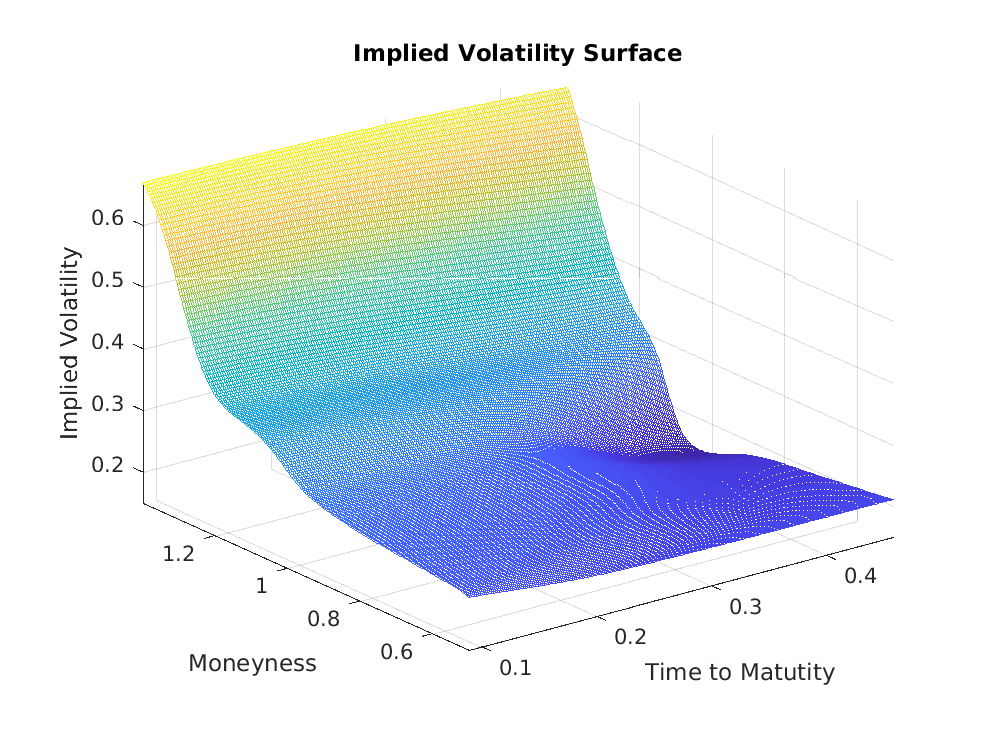
\includegraphics[scale=0.7]{figures/ivs_example.eps}
\end{center}
\vspace{-3mm}
\caption{\footnotesize Example of the fitted implied volatility surface on GOOG call options, 20150105 }
\label{ivsurf}
\end{figure}
\vspace*{\fill}

\newpage

\begin{figure}[H]
\begin{center}
 \minipage{0.45\textwidth}
 \includegraphics[width=\linewidth]{figures/hour_1th/GOOG_20150105_rnd_ci_1th_hour_ttm_1_07.png}
 \endminipage
 \hspace{3mm}
 \minipage{0.45\textwidth}
 \includegraphics[width=\linewidth]{figures/hour_1th/GOOG_20150105_iv_smile_1th_hour_ttm_1_07.png}
 \endminipage\\
 \minipage{0.45\textwidth}
 \includegraphics[width=\linewidth]{figures/hour_1th/GOOG_20150105_rnd_ci_1th_hour_ttm_1_3.png}
 \endminipage
 \hspace{3mm}
 \minipage{0.45\textwidth}
 \includegraphics[width=\linewidth]{figures/hour_1th/GOOG_20150105_iv_smile_1th_hour_ttm_1_3.png}
 \endminipage\\
 \minipage{0.45\textwidth}
 \includegraphics[width=\linewidth]{figures/hour_1th/GOOG_20150105_rnd_ci_1th_hour_ttm_1_53.png}
 \endminipage
 \hspace{3mm}
 \minipage{0.45\textwidth}
 \includegraphics[width=\linewidth]{figures/hour_1th/GOOG_20150105_iv_smile_1th_hour_ttm_1_53.png}
 \endminipage\\
 \minipage{0.45\textwidth}
 \includegraphics[width=\linewidth]{figures/hour_1th/GOOG_20150105_rnd_ci_1th_hour_ttm_2_47.png}
 \endminipage
 \hspace{3mm}
 \minipage{0.45\textwidth}
 \includegraphics[width=\linewidth]{figures/hour_1th/GOOG_20150105_iv_smile_1th_hour_ttm_2_47.png}
 \endminipage
\end{center}
\vspace{-3mm}
\caption{\footnotesize Risk-neutral densities and the corresponding implied volatility smiles obtained from call options on GOOG on 20150105, 1st hour of trading (9:30 - 10:30)} 
\label{rnd1}
\end{figure}

\newpage


\begin{figure}[H]
\begin{center}
 \minipage{0.45\textwidth}
 \includegraphics[width=\linewidth]{figures/hour_3th/GOOG_20150105_rnd_ci_3th_hour_ttm_1_07.png}
 \endminipage
 \hspace{3mm}
 \minipage{0.45\textwidth}
 \includegraphics[width=\linewidth]{figures/hour_3th/GOOG_20150105_iv_smile_3th_hour_ttm_1_07.png}
 \endminipage\\
 \minipage{0.45\textwidth}
 \includegraphics[width=\linewidth]{figures/hour_3th/GOOG_20150105_rnd_ci_3th_hour_ttm_1_3.png}
 \endminipage
 \hspace{3mm}
 \minipage{0.45\textwidth}
 \includegraphics[width=\linewidth]{figures/hour_3th/GOOG_20150105_iv_smile_3th_hour_ttm_1_3.png}
 \endminipage\\
 \minipage{0.45\textwidth}
 \includegraphics[width=\linewidth]{figures/hour_3th/GOOG_20150105_rnd_ci_3th_hour_ttm_1_53.png}
 \endminipage
 \hspace{3mm}
 \minipage{0.45\textwidth}
 \includegraphics[width=\linewidth]{figures/hour_3th/GOOG_20150105_iv_smile_3th_hour_ttm_1_53.png}
 \endminipage\\
 \minipage{0.45\textwidth}
 \includegraphics[width=\linewidth]{figures/hour_3th/GOOG_20150105_rnd_ci_3th_hour_ttm_2_47.png}
 \endminipage
 \hspace{3mm}
 \minipage{0.45\textwidth}
 \includegraphics[width=\linewidth]{figures/hour_3th/GOOG_20150105_iv_smile_3th_hour_ttm_2_47.png}
 \endminipage
\end{center}
\vspace{-3mm}
\caption{\footnotesize Risk-neutral densities and the corresponding implied volatility smiles obtained from call options on GOOG on 20150105, 3rd hour of trading (11:30 - 12:30)} 
\label{rnd2}
\end{figure}

\newpage


\begin{figure}[H]
\begin{center}
 \minipage{0.45\textwidth}
 \includegraphics[width=\linewidth]{figures/hour_5th/GOOG_20150105_rnd_ci_5th_hour_ttm_1_07.png}
 \endminipage
 \hspace{3mm}
 \minipage{0.45\textwidth}
 \includegraphics[width=\linewidth]{figures/hour_5th/GOOG_20150105_iv_smile_5th_hour_ttm_1_07.png}
 \endminipage\\
 \minipage{0.45\textwidth}
 \includegraphics[width=\linewidth]{figures/hour_5th/GOOG_20150105_rnd_ci_5th_hour_ttm_1_3.png}
 \endminipage
 \hspace{3mm}
 \minipage{0.45\textwidth}
 \includegraphics[width=\linewidth]{figures/hour_5th/GOOG_20150105_iv_smile_5th_hour_ttm_1_3.png}
 \endminipage\\
 \minipage{0.45\textwidth}
 \includegraphics[width=\linewidth]{figures/hour_5th/GOOG_20150105_rnd_ci_5th_hour_ttm_1_53.png}
 \endminipage
 \hspace{3mm}
 \minipage{0.45\textwidth}
 \includegraphics[width=\linewidth]{figures/hour_5th/GOOG_20150105_iv_smile_5th_hour_ttm_1_53.png}
 \endminipage\\
 \minipage{0.45\textwidth}
 \includegraphics[width=\linewidth]{figures/hour_5th/GOOG_20150105_rnd_ci_5th_hour_ttm_2_47.png}
 \endminipage
 \hspace{3mm}
 \minipage{0.45\textwidth}
 \includegraphics[width=\linewidth]{figures/hour_5th/GOOG_20150105_iv_smile_5th_hour_ttm_2_47.png}
 \endminipage
\end{center}
\vspace{-3mm}
\caption{\footnotesize Risk-neutral densities and the corresponding implied volatility smiles obtained from call options on GOOG on 20150105, 5th hour of trading (13:30 - 14:30)} 
\label{rnd3}
\end{figure}

\newpage

\begin{figure}[H]
\begin{center}
 \minipage{0.45\textwidth}
 \includegraphics[width=\linewidth]{figures/hour_7th/GOOG_20150105_rnd_ci_7th_hour_ttm_1_07.png}
 \endminipage
 \hspace{3mm}
 \minipage{0.45\textwidth}
 \includegraphics[width=\linewidth]{figures/hour_7th/GOOG_20150105_iv_smile_7th_hour_ttm_1_07.png}
 \endminipage\\
 \minipage{0.45\textwidth}
 \includegraphics[width=\linewidth]{figures/hour_7th/GOOG_20150105_rnd_ci_7th_hour_ttm_1_3.png}
 \endminipage
 \hspace{3mm}
 \minipage{0.45\textwidth}
 \includegraphics[width=\linewidth]{figures/hour_7th/GOOG_20150105_iv_smile_7th_hour_ttm_1_3.png}
 \endminipage\\
 \minipage{0.45\textwidth}
 \includegraphics[width=\linewidth]{figures/hour_7th/GOOG_20150105_rnd_ci_7th_hour_ttm_1_53.png}
 \endminipage
 \hspace{3mm}
 \minipage{0.45\textwidth}
 \includegraphics[width=\linewidth]{figures/hour_7th/GOOG_20150105_iv_smile_7th_hour_ttm_1_53.png}
 \endminipage\\
 \minipage{0.45\textwidth}
 \includegraphics[width=\linewidth]{figures/hour_7th/GOOG_20150105_rnd_ci_7th_hour_ttm_2_47.png}
 \endminipage
 \hspace{3mm}
 \minipage{0.45\textwidth}
 \includegraphics[width=\linewidth]{figures/hour_7th/GOOG_20150105_iv_smile_7th_hour_ttm_2_47.png}
 \endminipage
\end{center}
\vspace{-3mm}
\caption{\footnotesize Risk-neutral densities and the corresponding implied volatility smiles obtained from call options on GOOG on 20150105, 7th hour of trading (15:30 - 16:30)} 
\label{rnd4}
\end{figure}



\bibliographystyle{plainnat}
\bibliography{descriptive_sergey}


\end{document}


